\documentclass[12pt,fleqn]{article}\usepackage{../common}
\begin{document}
Kesit Seviyeleri, Kenar Bazli Imaj Gruplamak

Bir dijital imaji renklere, objelere gore belli parcalara bolmek
(segmentation) icin, matematiksel bir formul kullanmak iyi cozumlerden
biridir. Bunu yapmanin bazi yollari var. Basitlestirerek bir ornek
verelim: diyelim ki gruplama icin elimizdeki formul bir yuvarlak
formulu $x^2+y^2 - c = 0$, ki $c$ bir sabit. Bu formulu x ve y
kordinatlari uzerinde bastigimiz zaman radius'u $\sqrt{c}$ olan bir
cember elde ederiz. Gruplama icin bu cemberi buyutup
kucultebildigimizi farzedelim, cember imaj uzerindeki istedigimiz
bolume en iyi uydugu anda gruplamayi basarili olarak kabul ediyoruz.

Fakat problem surada: eger imajda birden fazla grup var ise, o zaman
birden fazla cember gerekecektir, bu sefer algoritmik olarak ustteki
formulu ikinci, ucuncu kere yaratmamiz, ve o formullerin o gruplara
uyumunu ayri ayri takip etmemiz gerekirdi. Ya da diyelim ki ozyineli
(iterative) bir uydurma islemi takip ediyoruz, bu islem sirasinda
belki iki cemberin birlesmesi gerekse, o zaman iki formulu silip,
yerine yenisini olusturmakla ugrasmak gerekli olacakti. Bunlar hem
matematiksel, hem kodlama acisindan kulfet olusturacaktir.

Kesit Seviyeleri kavramini kullanarak bu isi daha
basitlestirebiliriz. Diyelim ki bolme gorevini yapan $\phi$ adli
fonksiyonumuzu 2 boyutlu olmak yerine 3 boyutlu eksende tanimladik,
ve, 2 boyutta bolme yapma gorevini onun bir kesitine verdik. Kesit
derken, alttaki uc boyutlu fonksiyonu yatay olarak bir noktadan
``kestigimizi'' farz ediyoruz, ve o kesit uzerinde dusen $\phi$
degerlerine bakiyoruz.

Bakic acisimizi, tanimlamamizi degistirerek, bazi avantajlar elde
etmeyi umuyoruz aslinda. Altta iki tane $\phi$ fonksiyonu ve onlarin
altinda kesitlerini gorebiliriz.


Kesit Seviyeleri teknigini kullanarak elde ettigimiz avantaj nedir?
Artik sadece \textbf{tek} bir $\phi$ fonksiyonu kullanarak 2 boyutlu
imajimiz uzerinde birbirinden ayri gruplamalar yaratabiliyoruz. Bu
gruplar birbiri ile birlesebilir, ayrilabilir, bu artik bizi
ilgilendirmiyor. Biz sadece 3. boyuttaki $\phi$ fonksiyonunu
degistirmekle ugrasacagiz, imaj uzerindeki gruplamalar ise o
fonksiyonun 2. boyuta yansimasi (projection) uzerinden kendiliginden
gerceklesecekler.

Matematiksel olarak $\phi$ fonksiyonunu nasil temsil ederiz? $\phi$
fonksiyonu $x$, $y$, boyutlarini alip bize bir ucuncu $z$ boyutu
dondurmeli, ayrica bu fonksiyonu imaji parcalarina ayirma islemini
gerceklestirmek icin kademeli olarak degistirmeyi planladigimiza gore,
o zaman bir $t$ degiskeni de gerekiyor. Yani $\phi(x,y,t)$
fonksiyonu. Gruplama icin kullanilacak kesiti ise sifir kesiti olarak
alalim, yani $\phi(x,y,t) = 0$. Dogal olarak

\[ \frac{d}{dt}(\phi(x,y,t) = 0) = 0 \]

Simdi $x$, ve $y$ degiskenlerinin zaman gore degisimini formule bir
sekilde dahil etmek lazim. Bunun icin sifir kesit seviyesi uzerinde
bir parcacik hayal edilir, ve bu parcacigin gittigi yol $x(t)$, ve
$y(t)$ olarak tanimlanir. O zaman

\[ \frac{d}{dt}(\phi(x(t),y(t),t) = 0) = 0 \]

Tam diferansiyel formulunden hareketle:

\[ 
d(\phi(x(t),y(t),t) = 
\frac{\partial \phi}{\partial x}dx + 
\frac{\partial \phi}{\partial y}dy + 
\frac{\partial \phi}{\partial t}dt  = 0
 \]

\[ 
\frac{d(\phi(x(t),y(t),t))}{dt} = 
\frac{\partial \phi}{\partial x}\frac{dx}{dt} + 
\frac{\partial \phi}{\partial y}\frac{dy}{dt} + 
\frac{\partial \phi}{\partial t} = 0
 \]

\begin{equation} \frac{d(\phi(x(t),y(t),t))}{dt} = 
\frac{\partial \phi}{\partial x}\frac{dx}{dt} + 
\frac{\partial \phi}{\partial y}\frac{dy}{dt} + 
\phi_t = 0\label{eq1} 
\end{equation}

Temsilen daha kisa bir isaret kullanmak gerekirse, $\bigtriangledown$
ile $\phi$'nin gradyanini (gradient) alarak, elde edilecek vektorun
nokta carpimini kullanabiliriz.  O zaman formul~\ref{eq1} daha kisa
olarak:

\[ \phi_t + \bigtriangledown \phi \cdot \vec{V} = 0 \]

olarak temsil edilebilir, ki

\[ \bigtriangledown \phi = \bigg(
\frac{\partial \phi}{\partial x},
\frac{\partial \phi}{\partial y} \bigg)
 \]

\[ \vec{V} = \bigg(
\frac{dx}{dt} ,
\frac{dy}{dt} \bigg)
 \]

 Iki vektorun nokta carpimi bilindigi gibi sirayla her iki vektorun
 sirasiyla uyan elemanlarinin birbirleri ile carpilmasi ve o
 carpimlarin toplanmasidir.

$\vec{V}$ vektoru neyi temsil eder? Formule gore bu vektor $\phi$'nin
uzerindeki degisimi etkiliyor, ve bu degisimler $t$'nin degisimine
gore tanimlandigina gore bu degerler ``hiz'' olarak
tanimlanabilir. Imaj baglaminda dusunursek mesela $\phi$ renklerin
ayni oldugu yerlerde yuksek hizda, renklerin degistigi yerler dusuk
hizda degisebilir seklinde bir kurgu yapilabilir, iste bu bolgelerde
degisiminin hizini $\vec{V}$ ile gosterebiliriz.

$\vec{V}$ yerine kesit seviyelerine dik olan (normal) vektorler ile calismak
isteseydik, $\vec{V}$'yi dik ve teget bilesenlerine ayirarak tekrar temsil
edebilirdik: $\vec{V} = V_N\vec{N} + V_T\vec{T}$. Bu formulde $\vec{T}$ teget,
$\vec{N}$ dik vektorler, $N$ ve $T$ skalar. Yerine koyalim:

\[ \phi_t + \bigtriangledown \phi \cdot (V_N\vec{N} + V_T\vec{T}) = 0 \]

$\phi$'ye gore dik vektorun diger bir formulu $\vec{N} =
\frac{\bigtriangledown\phi}{|\bigtriangledown\phi|}$ olduguna gore

\[ \phi_t + (\bigtriangledown \phi \cdot
V_N\frac{\bigtriangledown\phi}{|\bigtriangledown\phi|} + \bigtriangledown
\phi \cdot V_T\vec{T}) = 0 \]

Devam edelim: $\bigtriangledown \phi$ yuzeye dik olduguna gore, bu dik vektorun
teget olan $\vec{T}$ ile noktasal carpimi sifir degerini verecektir, o carpim
formulden atilabilir. Kalanlar:

\[ \phi_t + (\bigtriangledown \phi \cdot 
V_N\frac{\bigtriangledown\phi}{|\bigtriangledown\phi|}) = 0 \]

Daha da kisaltabiliriz: $\bigtriangledown \phi \cdot \bigtriangledown
\phi = |\bigtriangledown \phi|^2$ oldugunu biliyoruz, gradyanin
kendisi ile noktasal carpimi, o gradyan vektorunun uzunlugunun
karesidir. Daha genel olarak, bir vektorun uzunlugu, o vektorun
kendisi ile noktasal carpiminin karekokudur. Ayni sey. O zaman en son
formulde bu carpimi gerceklestirip, uzunluk olarak yazalim:

\[ \phi_t + V_N\frac{|\bigtriangledown\phi|^2}{|\bigtriangledown\phi|} = 0  \]

\[ \phi_t + V_N |\bigtriangledown\phi| = 0  \]

Simdi bu formul hakkinda biraz anlayis gelistirelim. Eger elimizdeki
bir $\phi$ seviye kesitinin seklen oldugu gibi kalmasini ama sadece
kuculmesini isteseydik, $\phi$'nin normalinin tersi yonunde bir buyume
tanimlamamiz gerekirdi. Normal vektor disa dogru isaret ettigine gore
ustteki formulde mesela $V_N = -1$ tanimlayabilirdik. O zaman

\[ \phi_t + -1 |\bigtriangledown\phi| = 0 \]

\[ \phi_t = |\bigtriangledown\phi|   \]

Hesapsal olarak bunu nasil gerceklestiririz? 80 x 80 boyutunda bir
matris icinde $\phi$ fonksiyonu ayriksal olarak tutalim. Yani 80 tane
x, 80 tane ayri y degeri var, her x ve y degerlerin kombinasyonlarina
tekabul eden $\phi$ degerleri bu matris icinde. Gradyanin ne oldugunu
hatirlayalim. Gradyan

\[ 
\bigtriangledown \phi = \bigg(
\frac{\partial \phi}{\partial x},
\frac{\partial \phi}{\partial y} \bigg)
 \]

olarak tanimlidir, ve her $(x_i,y_i)$ noktasindaki $\phi(x_i,y_i)$
degerine gore degisik bir vektor sonucunu getirecektir. Bilgisayar
dunyasinda parcali turevler hesapsal ``farkliliklara'' donusurler,
\verb!phi! matrisindeki farkliliklari Python ile

\begin{lstlisting}[language=Python]
gradPhiY, gradPhiX = np.gradient(phi)    
\end{lstlisting}

olarak hesaplayabiliriz. Ustte elimize gecen gradyan dizinlerindeki
degerler ile $|\bigtriangledown\phi|$ buyuklugunu hesaplayabiliriz, ve bu
sonucu $\phi$ uzerindeki degisim orani $\phi_t$ olarak kabul ederiz. O
zaman $\phi_t$ ile zaman $t$ degimi \verb!dt! carptigimiz zaman ele gececek
olan $\phi$'nin degisimidir. Dongunun her basamaginda eski \verb!phi!
degerlerine bu farklari ekledigimiz zaman $\phi$ fonksiyonu istedigimiz
gibi evrilecektir.

Alttaki kodda bizim baslangic $\phi$'miz kenarlardan w uzakliginda ici bos
bir kutu olacak. Sifir seviyesindeki kesit seviyesinin nasil iki boyutlu
goruntudeki kirmizi cizgilere tekabul ettigini gorebiliriz.

\lstinputlisting[language=Python, frame=lines, caption=active1.py]{active1.py}

Ustteki kod isleyince sifir kesit seviyesinin (kirmizi cizgiler) olduklari
gibi kuculduklerini gorecegiz.

Ortalama Egim (Mean Curvature) Kullanmak

Eger sabit hiz yerine sifir kesit seviyesinin herhangi bir noktada ne kadar
``egri'' olduguna gore ilerlemesini isletseydik ne olurdu?  Diyelim ki cok
egri bolgelerde cok hizli, az egik (duz, duze yakin) bolgelerde ilerleme az
hiz istiyoruz. O zaman hangi sekille baslarsa baslasindalar $\phi$ kesiti
sonucta bir cember sekline dogru evrilecektir. Ortalama egim (mean
curvature) hesabi icin su denklem kullanilir:

\[ \kappa = -div \bigg( \frac{\bigtriangledown \phi}
{|\bigtriangledown \phi| } \bigg) \]

Bu formulun turetilmesini burada yapmayacagiz. Python kodu soyle:

\lstinputlisting[language=Python, frame=lines, caption=active2.py]{active2.py}

Imaj Gruplamak

Imaji bolumlere ayirmak icin (segmentation) birkac faktorun bilesimi
kullaniliyor. Koseleri kullanan aktif kontr (edge based active contour)
yonteminde ortalama egim ve imajin piksel degerlerinin farkliliklari (image
gradient) ayni anda kullanilir. Yani kesit seviyesini ilerletirken hizi hem
egime oranliyoruz, hem de imaj piksel renk degerleri arasindaki farka ters
oranda hizlandiriyor, ya da yavaslatiyoruz. Boylece kesit seviyemiz renk
farkliligi cok olmayan yani buyuk bir ihtimalle tek bir objeye ait bir
bolgede hizla ilerliyor, buyuk renk farkinin oldugu buyuk bir ihtimalle bir
kenar noktasina gelince ise yavasliyor. O sirada kesit seviyesinin geri
kalan taraflari tabii ki baska hizlarda hareket ediyor olabilirler, zaten
isin puf noktasi burada, sonunda resim bolgelere ayrilmis oluyor. Bu kodu
da \verb!active3.py! icinde bulabilir, \verb!active4.py! icinde ise surekli
degisim sonrasi sayisal bazi yan etkilerden dolayi $\phi$'nin dejenere
olmasi sonucu onu ``tekrar bastan olusturan (reinitialization)'' iceren bir
kisim var. Fakat teknigin ozu her iki kod icinde de gorulebilir.

Bitirirken onemli gozlemi vurgulayalim. Problemi matematiksel olarak temsil
ederken, hedefe dogru turetirken surekli (continous) alemde, surekli,
kesintisiz fonksiyonlarla is yapiyoruz. Hesaplama ani gelince surekli
fonksiyonlari ayriksal (discrete) hale ceviriyoruz, iste uygulamali
matematigin hesapsal kismi burada devreye giriyor. Fakat diferansiyel
denklemler, fonksiyonlar, turevler gibi surekli matematigin kavramlari cok
onemli, bunlar olmasa problemi soyut bir sekilde temsil edemez, ve
basitlestiremezdik. Temel matematigin kavramlarini kullanirken yuzyillarin
matematiksel bilgisi devreye girebiliyor, matematigin en yogun sekilde
kullanildigi fizikten bol bol teknik alinabilir. Yani soylemek istedigimiz
problemi cozmek icin hemen kodlamaya baslamiyoruz, dusunsel eylemin onemli
bir kismi matematiksel formullerle (belki kalem kagitla) yapiliyor.

\lstinputlisting[language=Python, frame=lines, caption=active3.py]{active3.py}

\lstinputlisting[language=Python, frame=lines, caption=active4.py]{active4.py}

\lstinputlisting[language=Python, frame=lines, caption=plot\_phi.py]{plot_phi.py}

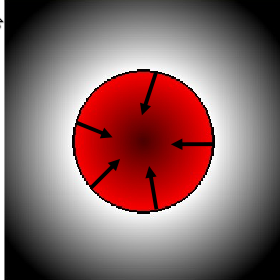
\includegraphics[height=4cm]{pics/inwards.png}

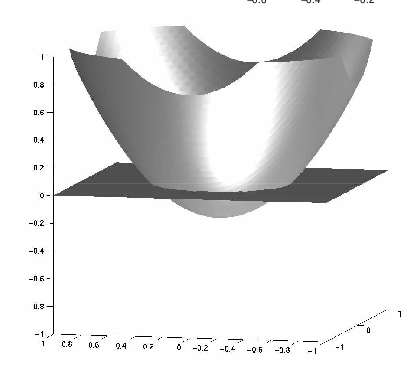
\includegraphics[height=4cm]{pics/level1.png}

$\phi$ Fonksiyonu

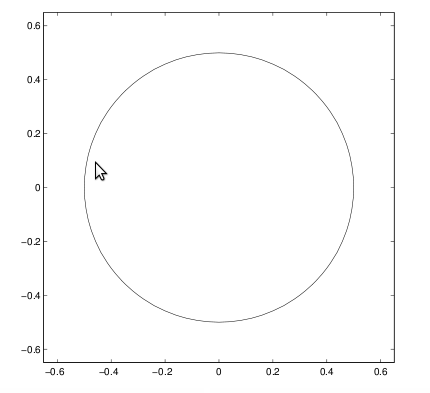
\includegraphics[height=4cm]{pics/level2.png}

Kesit Seviyesi

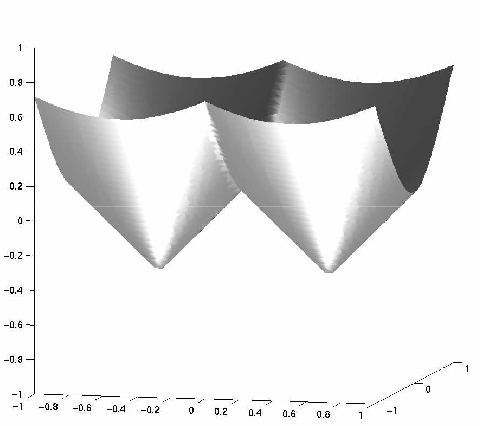
\includegraphics[height=4cm]{pics/level3.png}

$\phi$ Fonksiyonu

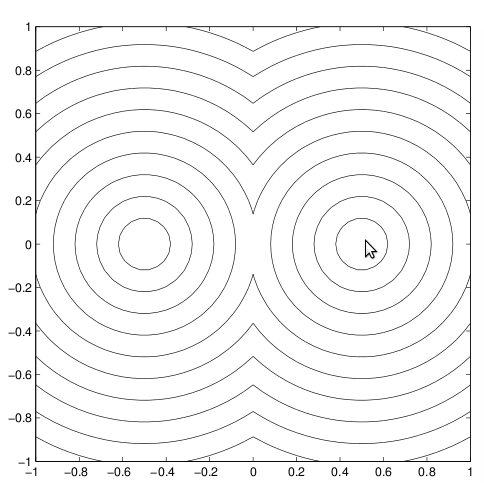
\includegraphics[height=4cm]{pics/level4.png}

Birkac z Seviyesinden Kesitler

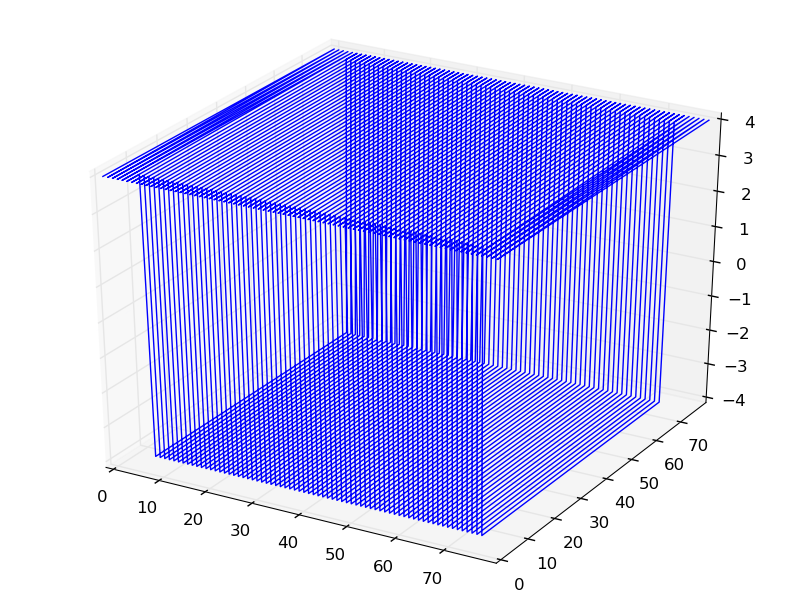
\includegraphics[height=4cm]{pics/phi_init.png}

$\phi$ Baslangici

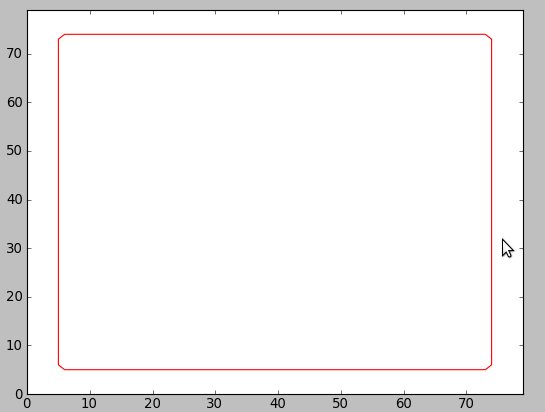
\includegraphics[height=4cm]{pics/phi_init_2d.png}

$\phi$ Baslangici 2 Boyutta

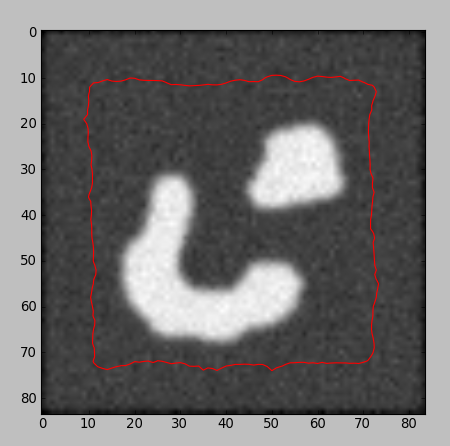
\includegraphics[height=7cm]{pics/edge1.png}

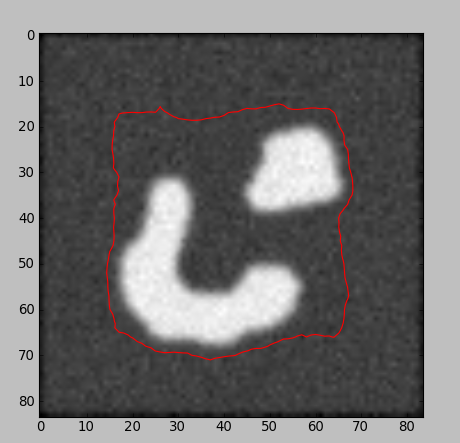
\includegraphics[height=7cm]{pics/edge2.png}

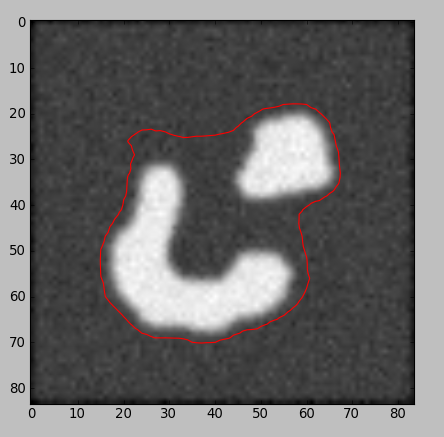
\includegraphics[height=7cm]{pics/edge3.png}

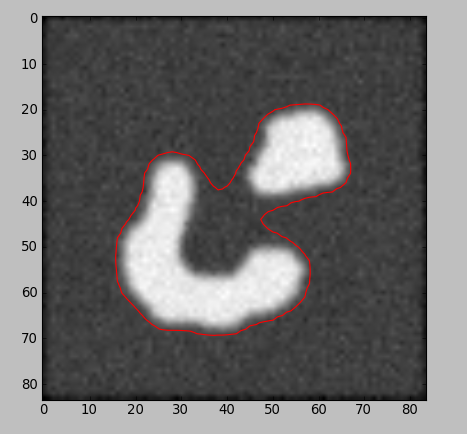
\includegraphics[height=7cm]{pics/edge4.png}

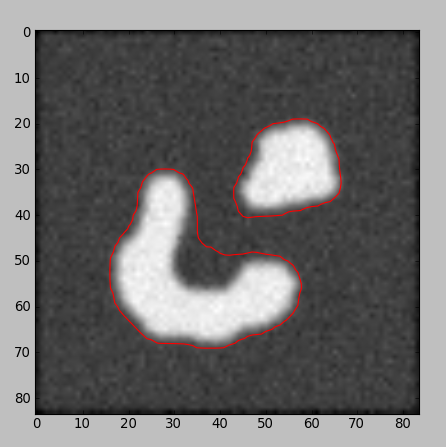
\includegraphics[height=7cm]{pics/edge5.png}

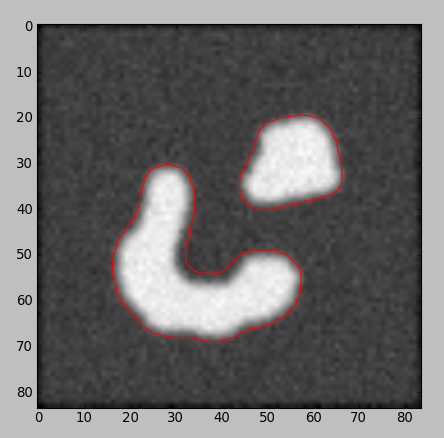
\includegraphics[height=7cm]{pics/edge6.png}


\end{document}
